\section{Results}
In this section, we first compare the number of GMRES iterations needed by
ANMG-DSA and ANMG-$P1$SA to solve a model problem. Then, both the number of
GMRES iterations and the elapsed time are compared for three methods:
\begin{itemize}
  \item Sweep preconditioning (S).
  \item DSA preconditioning (DSA).
  \item Angular multigrid (DSA variant) preconditioning (ANMG-DSA).
\end{itemize}
For all the tests the first in this section, BLD finite elements are used and GMRES is
restarted every 30 iterations. For the comparison between ANMG-DSA and
ANMG-$P1$SA GMRES is restarted every 20 iterations.
\subsection{Comparison between ANMG-DSA and ANMG-$P1$SA}
The test uses a 5$cm$ square domain, uniformly discretized using $50 \times
50$ cells. The homogeneous medium is homogeneous with an uniform isotropic source of
intensity $10 n/(cm^3 s)$ and Fokker-Planck cross sections with $\alpha=1$. 
$\Sigma_t$ is chosen to be equal to $\Sigma_{s,0}$. The quadrature is the 
Gauss-Legendre-Chebyshev triangular Galerkin quadrature. The GMRES solver is 
converged to a relative tolerance, $\(\frac{\|\textrm{residual}\|_2}{\|\textrm{right 
hand side}\|_2}\)$, of $10^{-4}$. $P1$SA is solved using BiCGSTAB with a relative 
tolerance of $10^{-6}$. DSA is solved with CG preconditioned by an algebraic 
multigrid technique \cite{pyamg,amg} with a relative tolerance of $10^{-6}$. The 
number of GMRES iterations needed to solve ANMG-DSA (multigrid preconditioner 
with $S_2$ as coarsest transport level and diffusion solve) and ANMG-$P1$SA 
(multigrid preconditioner with $S_4$ as coarsest transport level and $P1$SA solve) 
are compared, see Table \ref{table_anmg_d_p1}. The comparison is performed for 
$S_4$, $S_8$ and $S_{16}$ (for which the values of the anisotropy order $L$ are 4, 
8, 16, respectively).
\begin{table}[H]
  \begin{center}
    \caption{Comparison of the number of GMRES iterations needed in ANMG-DSA
    and ANMG-$P1$SA}
    \begin{tabular}{|c|c|c|}
      \hline
      & ANMG-DSA & ANMG-$P1$SA \\
      \hline
      $S_4$ & 17 & 15 \\
      $S_8$ & 23 & 28 \\
   $S_{16}$ & 42 & 70 \\
      \hline
    \end{tabular}
  \label{table_anmg_d_p1}
  \end{center}
\end{table}
From Table \ref{table_anmg_d_p1}, it can be seen that ANMG-DSA outperforms
ANMG-$P1$SA except for $S_4$. When the anisotropy of the problem increases,
the advantage of ANMG-DSA over ANMG-$P1$SA increases. Furthermore, we note
that the $P1$SA equations are more difficult to solve (PD but non symmetric
system) than the DSA equations (which are SPD). For these reasons, we
recommend using the ANMG-DSA variant of the angular multigrid technique.
Consequently, only the ANMG-DSA method will be employed in the later tests.
\subsection{Test Case with a Volumetric Source}
In this test, we compare ANMG-DSA to Sweep and DSA preconditioning. An uniform
isotropic source of intensity 10 $n/(cm^3 s)$. $S_4$, $S_8$, $S_{16}$, and
$S_{32}$ calculations were performed. Fokker-Planck cross sections with
$\alpha=1$ are used and $\Sigma_t = \Sigma_{s,0}$ $(c=1)$. The domain is homogeneous
and its size is $50cm \times 50cm$ discretized by $50\times 50$ cells. The 
thickness of the domain varies from 50 to 2690 mean-free-path (the total cross 
section varies with $L$ for Fokker-Planck cross sections: $\Sigma_{t,S_4}=10cm^{-1},
\Sigma_{t,S_8}=36cm^{-1}, \Sigma_{t,S_{16}}=136cm^{-1}, 
\Sigma_{t,S_{32}}=528cm^{-1}$) but stays constant at five transport
mean-free-path. The relative tolerance on GMRES, which is restarted every 30
iterations, is $10^{-6}$ whereas the
relative convergence on DSA, solved by AGMG (see next Chapter), is $10^{-8}$.
The solution for $S_{32}$ calculation is given on Figure \ref{fig_s_32}
\begin{figure}[H]
  \centering
  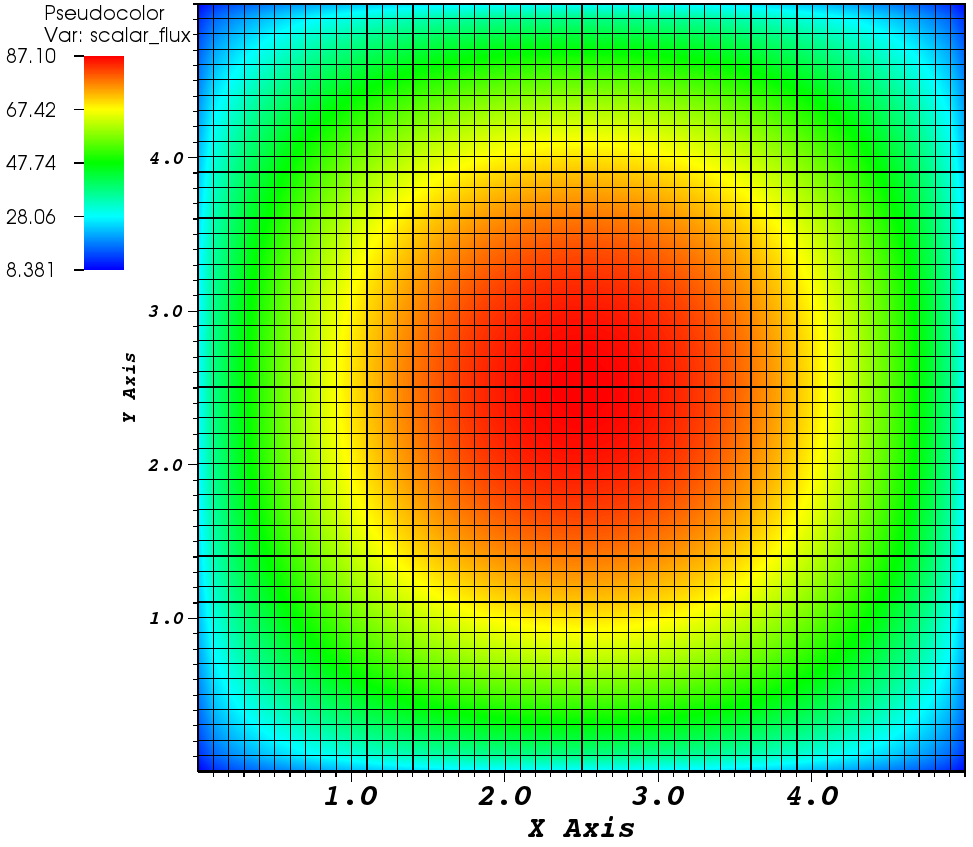
\includegraphics[width=0.6\textwidth]{Anmg/homog_anmg_crop}
  \caption{Scalar flux for the $S_{32}$ calculation on a homogeneous medium}
  \label{fig_s_32}
\end{figure}
\begin{table}[H]
  \begin{center}
    \caption{Comparison of the number of GMRES iterations needed to solve the 
      volumetric source test problem when $c=1$ using sweep preconditioning (S), DSA 
    preconditioning, and ANMG-DSA preconditioning on a homogeneous medium}
    \begin{tabular}{|c|c|c|c|c|}
      \hline
      & S & DSA & ANMG-DSA & $\frac{\textrm{DSA}}{\textrm{ANMG-DSA}}$ \\
      \hline
      $S_4$ & 85   & 42  & 27  & 0.64 \\
      $S_8$ & 409  & 102 & 50  & 0.49 \\
   $S_{16}$ & 1530 & 266 & 105 & 0.39 \\
   $S_{32}$ & 4535 & 616 & 225 & 0.36 \\
      \hline
    \end{tabular}
    \label{table_gmres_homog}
  \end{center}
\end{table}
\begin{table}[H]
  \begin{center}
    \caption{Elapsed time (s) to solve the volumetric source test problem when
      $c=1$ using sweep preconditioning (S), DSA preconditioning, and ANMG-DSA
    preconditioning on a homogeneous medium}
    \begin{tabular}{|c|c|c|c|c|}
      \hline
      & S & DSA & ANMG-DSA & $\frac{\textrm{DSA}}{\textrm{ANMG-DSA}}$ \\
      \hline
      $S_4$ & 9.09322 & 6.51608 & 5.22796 & 0.80 \\
      $S_8$ & 184.949 & 52.65   & 32.7609 & 0.62 \\
   $S_{16}$ & 4610.94 & 740.193 & 355.939 & 0.48 \\
   $S_{32}$ & 138181  & 17907.9 & 7357.63 & 0.41 \\
      \hline
    \end{tabular}
    \label{table_time_homog}
  \end{center}
\end{table}
In Table \ref{table_gmres_homog}, one can note that ANMG-DSA always
requires the least number of iterations to converge. ANMG is the fastest
method (Table \ref{table_time_homog}). It took 38 hours to solve the $S_{32}$
problem with sweep preconditioning but only 2 hours when ANMG-DSA was used. As 
the anisotropy order is increased (i.e., increasing values of $L$ as a function 
of the number of directions in the Fokker-Planck cross-section representation), 
the advantage of ANMG-DSA is clear. The ratio $\(\frac{\textrm{number of GMRES 
iterations for ANMG-DSA}}{\textrm{number of GMRES iterations for DSA}}\)$ and
the ratio of elapsed times between the DSA and the ANMG-DSA
techniques decrease monotonically. We note from these results that
ANMG-DSA becomes increasingly superior to the standard DSA as the number of
directions becomes larger.
\subsection{Test Case with a Heterogeneous Medium (Beam problem)}
In this test, we apply a boundary source of intensity 10 $n/(cm^2 s)$ to the
entire left side of the domain $y \in [0cm,5cm]$. The top, the bottom, 
and the right boundary conditions are vacuum. The beam intensity is only 
non-zero in the most-normal directions of the quadrature. An $S_{16}$ Galerkin 
Gauss-Legendre-Chebyshev quadrature is used. The domain
is discretized using $50 \times 50$ cells and is composed of two materials:
\begin{description}
  \item[Material 1:] for $x\in [0cm,3cm]$, Fokker-Planck cross section is used with 
    $\alpha=0.099$, $\Sigma_t = 13.6 cm^{-1}$, $c=0.99$
  \item[Material 2:] for $x\in [3cm,5cm]$, Fokker-Planck cross section is used with 
    $\alpha=9.999$, $\Sigma_t = 1360 cm^{-1}$, $c=0.99$
\end{description}
Like previously, the relative tolerance on GMRES, which is restarted every 30
iterations, is $10^{-6}$ and the relative tolerance on DSA is $10^{-8}$. 
\begin{figure}[H]
  \centering
  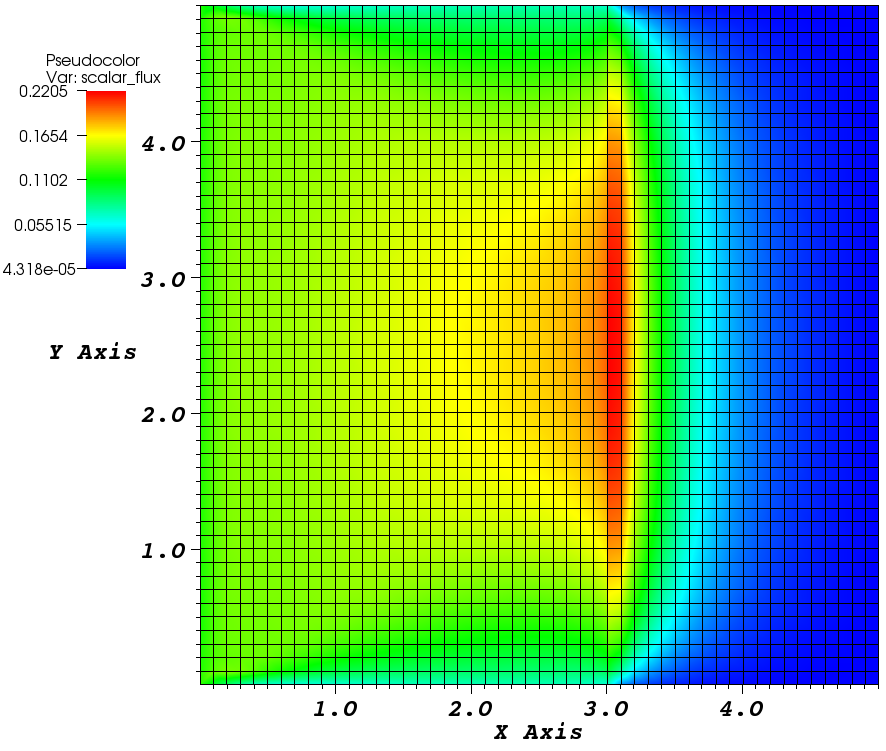
\includegraphics[width=0.6\textwidth]{Anmg/heterog_anmg_crop}
  \caption{Scalar flux for the $S_{32}$ calculation on a heterogeneous medium}
\end{figure}
The number of GMRES iterations and the elapsed 
time are given in Table \ref{table_gmres_heter} and Table \ref{table_time_heter}.
\begin{table}[H]
  \begin{center}
    \caption{GMRES iterations to solve the heterogeneous problem using sweep
    preconditioning (S), DSA preconditioning, and ANMG-DSA preconditioning on
    a heterogeneous medium}
    \begin{tabular}{|c|c|c|}
      \hline
      S & DSA & ANMG-DSA \\
      \hline
      5001 & 283 & 96 \\
      \hline
    \end{tabular}
    \label{table_gmres_heter}
  \end{center}
\end{table}
\begin{table}[H]
  \begin{center}
    \caption{Elapsed time (s) to solve the heterogeneous problem using sweep
    preconditioning (S), DSA preconditioning, and ANMG-DSA preconditioning on
    a heterogeneous medium}
    \begin{tabular}{|c|c|c|}
      \hline
      S & DSA & ANMG-DSA \\
      \hline
      13642.8 & 897.072& 394.965 \\
      \hline
    \end{tabular}
    \label{table_time_heter}
  \end{center}
\end{table}
We can see that even on a heterogeneous medium the angular multigrid is the
most effective. The sweep preconditioning method requires significantly more
iterations than DSA and ANMG-DSA preconditioning because of the Material 2
which is very thick and a scattering ratio close to one.
